\section{Derivation: Basic Model}
\label{section:derivation:basic_model}
\begin{enumerate}
    \item Let $\tau_s$ be the synaptic time constant of each synapse in the network. Define dimensionless time as:
    \begin{equation*}
        \xi \overset{\Delta}{=} \frac{t}{\tau_s}.
    \end{equation*}\\
    We now assume our Linear Dynamical System is expressed in dimensionless time, i.e
    
    \begin{equation}
        \label{eq:lds_dimensionless}
        \frac{dx}{d\xi} = Ax(\xi) + B c(\xi).
    \end{equation}
    
    To describe the neuron dynamics in dimensionless time, let $o(\xi) \in \mathbf{R}^{N}$ be the spike trains of N neurons composing the network with components
    \begin{equation*}
        o_j(\xi) = \sum_{k=1}^{\text{$n_j$ spikes}} \delta(\xi - \xi_{j}^{k}),
    \end{equation*}
    where $\xi_j^k$ is the time at which neuron $j$ makes its $k^{th}$ spike. 
    Define the network's estimate of the state variable as
    \begin{equation}
        \label{eq:xhat}
        \hat{x}(\xi)
        \overset{\Delta}{=} D r(\xi), 
    \end{equation}
    where $D \in \mathbf{R}^{d \times N}$ and 
    \begin{equation}
    \label{eq:rdot}
        \frac{dr}{d \xi} = -r + o(\xi).
    \end{equation}\\
    When the probability of synaptic transmission is $1$, component $r_j$ is the total received post-synaptic current (PSC) from neuron $j$ by the network estimator. 
    Define the network error as
    \begin{equation}
    \label{eq:error_def}
        e(\xi) \overset{\Delta}{=} x(\xi) - \hat{x}(\xi).
    \end{equation}
    
    \item From equations (\ref{eq:rdot}) and (\ref{eq:xhat}), we have
    
    \begin{align*}
        D \dot{r} + D r &= Do \\
        \\
        \implies \dot{\hat{x}} + \hat{x} &= Do,
    \end{align*}
    where the dot denotes derivative w.r.t dimensionless time $\xi$.

    Subtract $\dot{\hat{x}}$ from $\dot{x}$ to get $\dot{e}$:
    \begin{align}
    \label{eq:derivation_init}
        \dot{e} &= \dot{x}-\dot{\hat{x}} \notag \\
        &= \left( Ax + Bc \right) - \left( Do - \hat{x} \right) \notag \\
        &= A\left(  e + \hat{x} \right) + Bc - Do + \hat{x} \notag \\
        &= A e + (A + I)\hat{x} + Bc - Do \notag \\
        &=  A e + (A + I) \left(Dr\right) + Bc - Do \notag \\
        \implies A^{-1}\dot{e} &= e + (I + A^{-1}) Dr + A^{-1} Bc - A^{-1}Do \notag \\ 
        \implies D^{T} A^{-1} \dot{e} &= D^T e +D^T (I + A^{-1}) Dr + D^T A^{-1}Bc - D^T A^{-1} D o 
    \end{align}
where the third equality follows from equation (\ref{eq:error_def}) and the fifth from equation (\ref{eq:xhat}).    

\item Assuming both $D$ and $A$ are full rank, diagonalize each to a common left basis:
\begin{align*}
    A &= \mathcal{U} \Lambda \mathcal{U}^T = \sum_{j=1}^d \Lambda_j \mathcal{U}_j \mathcal{U}_j^T,\\
    \\
    D &= \mathcal{U} \left[S \hspace{2mm} 0 \right]  V^T = \sum_{j=1}^d S_j \mathcal{U}_j  V_j^T,\\
    \\
    D^T &= V \begin{bmatrix} S \\ 0\end{bmatrix} \mathcal{U}^T = \sum_{j=1}^d S_j V_j  \mathcal{U}_j^T, \\
    \\
    D^T D  &= V \begin{bmatrix} S \\ 0\end{bmatrix} \begin{bmatrix} S & 0\end{bmatrix} V^T
     = \sum_{j=1}^d S_j^2 V_j V_j^T , 
\end{align*}
with $\mathcal{U} \in \mathbf{R}^{d \times d}$ and $V \in \mathbf{R}^{N \times N}$, and $S \in \mathbf{R}^{d \times d }$. \\
\\
To express equation (\ref{eq:derivation_init}) with the $\mathcal{U}$ and $V$ bases, first note

\begin{align*}
     D^{T} A^{-1}  &= V \begin{bmatrix} S \\ 0\end{bmatrix} \mathcal{U}^T  \mathcal{U} \Lambda^{-1} \mathcal{U}^T \\
     &= V \begin{bmatrix} S \\ 0\end{bmatrix} \Lambda^{-1} \mathcal{U}^T \\
     &= \sum_{j = 1}^{d} \frac{S_j}{ \Lambda_j} V_j \mathcal{U}_j^T,
\end{align*}\\

and

\begin{align*}
D^{T} A^{-1} D  &= V \begin{bmatrix} S \\ 0\end{bmatrix} \mathcal{U}^T  \mathcal{U} \Lambda^{-1} \mathcal{U}^T \mathcal{U} \left[S \hspace{1mm} 0 \right] V^T \\
  &= V \begin{bmatrix} S \\ 0\end{bmatrix} \Lambda^{-1} \left[S \hspace{1mm} 0 \right] V^T \\
  &= \sum_{j = 1}^{d} \frac{S_j^2}{ \Lambda_j} V_j V_j^T.
\end{align*}

Consequently, 

\begin{align}
    \label{eq:derivation_sub_svd}
    \sum_{j = 1}^{d} \frac{S_j}{ \Lambda_j} V_j \mathcal{U}_j^T \dot{e} &= 
     \sum_{j=1}^d S_j V_j  \mathcal{U}_j^T e
    +
    \sum_{j = 1}^{d} S_j^2 (1 + \Lambda_j^{-1}) V_j V_j^T r
    + 
    \sum_{j = 1}^{d} \frac{S_j}{ \Lambda_j} V_j \mathcal{U}_j^TBc 
    -
    \sum_{j = 1}^{d} \frac{S_j^2}{ \Lambda_j} V_j V_j^T o.
\end{align}


Left-multiply both sides of the preceding equation by $V_j^T$ to arrive at the system of equations

\begin{align*}
    \frac{S_j}{\Lambda_j} \mathcal{U}_j^T \dot{e} &= 
    S_j \mathcal{U}_j^T e
    +
    S_j^2 (1 + \Lambda_j^{-1})V_j^T r 
    +
    S_j \Lambda_j^{-1} \mathcal{U}_j^T B c
    -
    S_j^2 \Lambda_j^{-1} V_j^T o
    \\
    \\
    \implies 
    \mathcal{U}_j^T \dot{e} 
    &= 
    \Lambda_j \mathcal{U}_j^T e
    +
    S_j(\Lambda_j + 1) V_j^T r 
    +
    \mathcal{U}_j^T B c
    -
    S_j V_j^T o,\\
\end{align*}
for $j = 1, \ldots, d$.

\item To simplify notation, we note that our preceding left-multiply has transformed the equations to the basis $V^T$. The transformed neuron's fast synaptic inhibition (reset), membrane voltage, slow synaptic excitation, and input weight vector are respectively: 
\begin{align}
    \label{eq:rotated_voltage_psc_def}
    \Omega_j \overset{\Delta}{=} S_j V_j^T o \notag \\  \notag 
    \\  \notag 
    v_j \overset{\Delta}{=} 
    \mathcal{U}_j^T e, \notag  \\
    \\
    \rho_j \overset{\Delta}{=} S_j V_j^T r  \notag \\  \notag 
    \\  \notag 
    \beta_j \overset{\Delta}{=} \mathcal{U}_j^T B. \notag 
\end{align}

The system of equations simplifies to the membrane voltage dynamics
\begin{align*}
    \dot{v}_j &= 
    \Lambda_j v_j
    +
    (\Lambda_j + 1) \rho_j 
    +
     \beta_j c
    -
   \Omega_j,\\
\end{align*}

or in matrix form,

\begin{align}
\label{eq:rotated_voltage_dynamics}
    \dot{v} &= 
    \Lambda v
    +
    (\Lambda + I) \rho 
    +
     \beta c
    -
   \Omega.
   \end{align}
   \\
Here, $v$ is a d vector which describes the dynamics of the d-neurons needed to implement the dynamical system. The remaining $N-d$ neurons are unused and do not contribute to the network readout at present.   \\
From equation (\ref{eq:rdot}) the PSC dynamics are
\begin{equation}
\label{eq:rho_dot}
    \dot{\rho} = -\rho + \Omega.
\end{equation}
Similar to equation (\ref{eq:rotated_voltage_dynamics}), $\rho$ describes a d-vector. 

 
   
   
\item The spike trains are chosen minimize the network estimation error
\begin{align}
    \mathcal{L}(\xi) =  || x(\xi + d\xi) - \hat{x}(\xi + d\xi) ||^2. 
\end{align}
The network greedily minimizes $\mathcal{L}$ an instant $d\xi$ ahead in time. Writing $\hat{x}$ in terms of $\Omega$ and $\rho$, equations (\ref{eq:xhat}) and (\ref{eq:rotated_voltage_psc_def}) imply 

\begin{align*}
    \hat{x} &= D r 
    \\
    \\
    &=
    \sum_{j=1}^d S_j \mathcal{U}_j V_j^T r
    \\
    \\
    &= 
    \sum_{j=1}^d \mathcal{U}_j \rho_j
    \\
    \\
    &=
    \mathcal{U} \rho. 
\end{align*}

If neuron $j$ does not spike, the objective is
\begin{align*}
    \mathcal{L}_{ns} = ||x - \hat{x}||^2.
\end{align*}
 
If neuron $j$ spikes at time $\xi$, then $\hat{x} \leftarrow \hat{x} + \hat{U}_j$. The objective is now
\begin{align*}
    \mathcal{L}_{sp} &= || x - (\hat{x} + \mathcal{U}_j) ||^2,\\
    \\
    &= 
    (x-\hat{x}-\mathcal{U}_j)^T (x-\hat{x}-\mathcal{U}_j)\\
    &= 
    x^T x - x^T \hat{x} - x^T \mathcal{U}_j
    - \hat{x}^T x +\hat{x}^T\hat{x} +\hat{x}^T \mathcal{U}_j
    -
    \mathcal{U}_j^T x + \mathcal{U}_j^T \hat{x} + \mathcal{U}_j^T \mathcal{U}_j
    \\
    &=
    \left(x^T x -2 x^T \hat{x} +\hat{x}^T\hat{x}  \right) + 
    2 \mathcal{U}_j^T \left( \hat{x} - x
    \right) + \mathcal{U}_j^T \mathcal{U}_j\\
    &= 
    ||x -\hat{x}|| +  2 \mathcal{U}_j^T \left( \hat{x} - x
    \right) + \mathcal{U}_j^T \mathcal{U}_j\\
    &= 
    \mathcal{L}_{ns} + 2 \mathcal{U}_j^T \left( \hat{x} - x
    \right) + \mathcal{U}_j^T \mathcal{U}_j\\
\end{align*}
 A spike occurs when it lowers the objective more than not spiking. Our spiking condition is therefore
\begin{align*}
    \mathcal{L}_{sp} &< \mathcal{L}_{ns}\\
    \\
    \implies
     2 \mathcal{U}_j^T \left( \hat{x} - x
    \right) &+ \mathcal{U}_j^T \mathcal{U}_j < 0\\
    \\
    \implies 
    \mathcal{U}_j^T \left(x -\hat{x} \right) &> \frac{\mathcal{U}_j ^T \mathcal{U}_j}{2}\\
    \\
    \implies
    \mathcal{U}_j^T e &> \frac{\mathcal{U}_j^T \mathcal{U}_j}{2}
    \\
    \\
    \implies
    v_j &> \frac{1}{2},
\end{align*}
where the last inequality follows from applying the voltage definition from equation ($\ref{eq:rotated_voltage_psc_def}$). Thus neuron $j$ spikes when its membrane voltage $v_j$ exceeds the threshold of $v_{th} = \frac{1}{2}$. 

\item Equations (\ref{eq:rotated_voltage_dynamics}) and (\ref{eq:rho_dot}) describe how we implement a network with d neurons that produces an accurate estimate $\hat{x}$ of the given target system. 


When neuron $j$ spikes, a vector $\mathcal{U}_j$ is added to the network estimate, $\hat{x}$. A spike has a strictly positive area so that the network is only able to modify its estimate by adding from a fixed set of vectors.  This restricts the space representable by the network to strictly positive state-space, or only $\frac{1}{2^d}$ of the desired state-space. To remove this restriction, we add an additional d neurons whose preferred directions $\mathcal{U}_j$ are anti-parallel to neurons $j$ for $j=1, \ldots, d$. Such vectors are required in order to allow subtraction, defined as addition of the additive inverse. Thus the number of neurons required to represent a d-dimensional system is $2d$. We update $U$, $S$, $\Lambda$ and $v_{th}$ to reflect the additional neurons:
\begin{align*}
    U &\leftarrow \left[ U \hspace{2mm} -U\right] \in \mathbf{R}^{d \times 2 d},\\
    \\
    S &\leftarrow
    \begin{bmatrix}
    S & 0 \\ 0 & S
    \end{bmatrix}
    \in \mathbf{R}^{2 d \times 2 d},\\
    \\
    \Lambda &\leftarrow
    \begin{bmatrix}
    \Lambda & 0 \\ 0 & \Lambda
    \end{bmatrix}
    \in \mathbf{R}^{2 d \times 2 d},\\
    \\
    v_{th} &\leftarrow 
    \begin{bmatrix}
    v_{th} \\ v_{th}
    \end{bmatrix} \in \mathbf{R}^{2d},
\end{align*}
and afterward recompute $\beta \in \mathbf{R}^{2 d \times d}$. 

\end{enumerate}

\textbf{\textit{Simulation of Basic Equations}}\\
\\
Here we simulate the above equations (\ref{eq:rotated_voltage_dynamics}) and (\ref{eq:rho_dot}) with the $N = 2d$ neurons. The parameters are
\begin{align}
\label{eq:sim_I_params}
A
&=
\ -\begin{bmatrix}  
1 & 0 \\
0 & 1
\end{bmatrix} = \mathcal{U} \Lambda \mathcal{U}^T \notag,
\\
\notag
\\
B
&=
\begin{bmatrix}  
1 & 0 \\
0 & 1
\end{bmatrix}, \notag 
\\
\notag 
\\
c(\xi) 
&=
10 \begin{bmatrix} 
cos(\frac{\pi}{4} \xi)\\
sin(\frac{\pi}{4} \xi)
\end{bmatrix} 
\\
\notag
\\
D
&=
\mathcal{U} 
\begin{bmatrix}
S & 0
\end{bmatrix}
V^T
=
\mathcal{U} 
\begin{bmatrix}
I_d & 0
\end{bmatrix}
I_N \notag,
\\
\notag 
\\
d\xi 
&= 
10^{-6}, \notag 
\\
\notag 
\\
N 
&= 
4,\notag 
\\
\notag 
\\
x(0) 
&= 
\begin{bmatrix} \frac{1}{2} & \frac{1}{2} \end{bmatrix}.\notag 
\end{align}

\begin{figure}
    \centering
    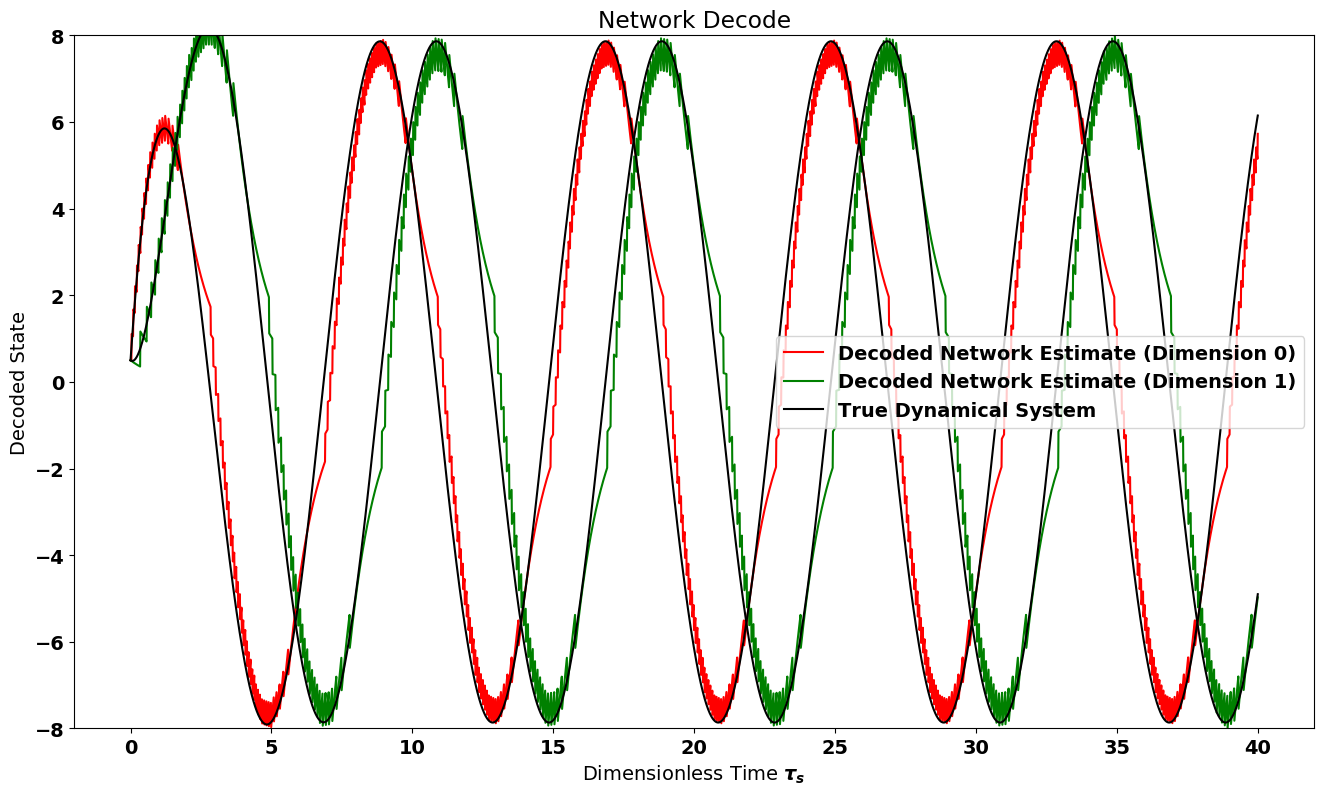
\includegraphics[width=.75\linewidth]{figures/network_decode.png}

    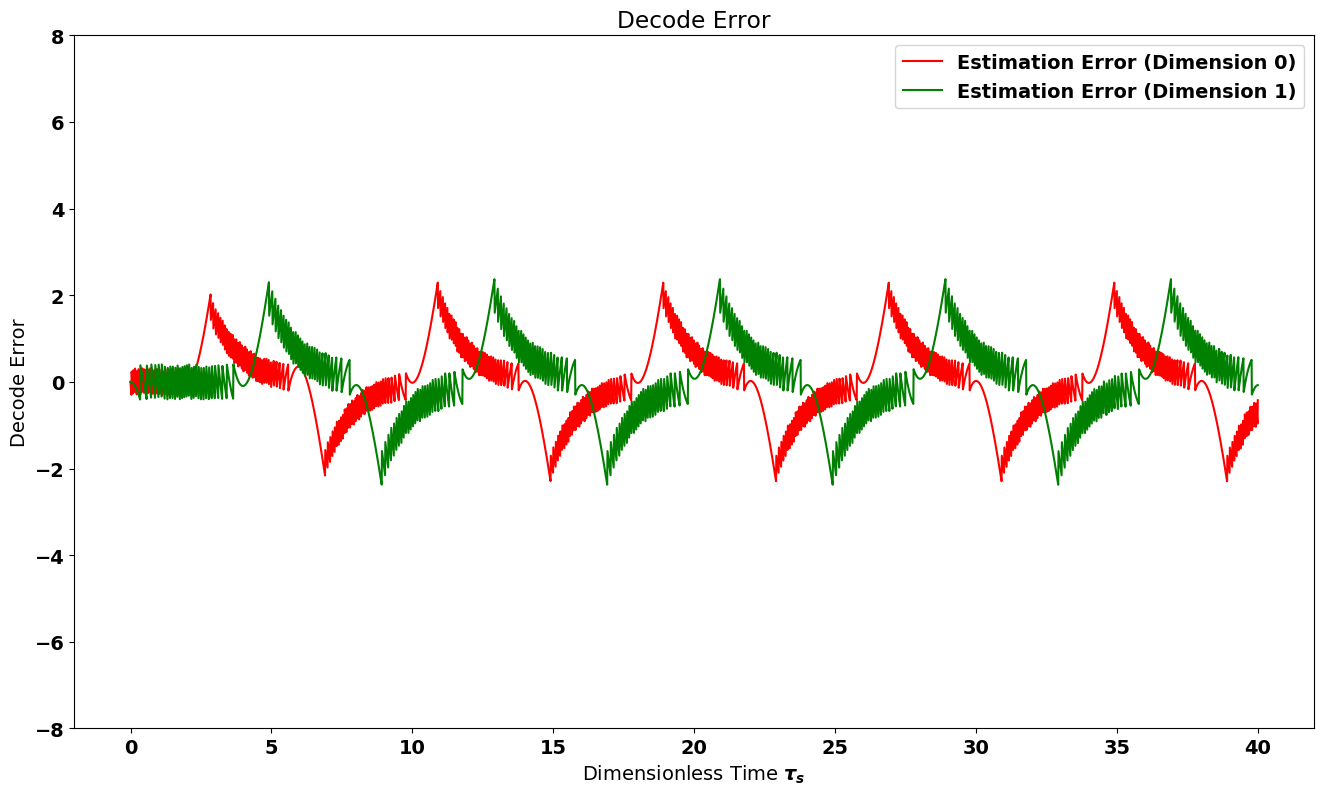
\includegraphics[width=.75\linewidth]{figures/decode_error.png}

    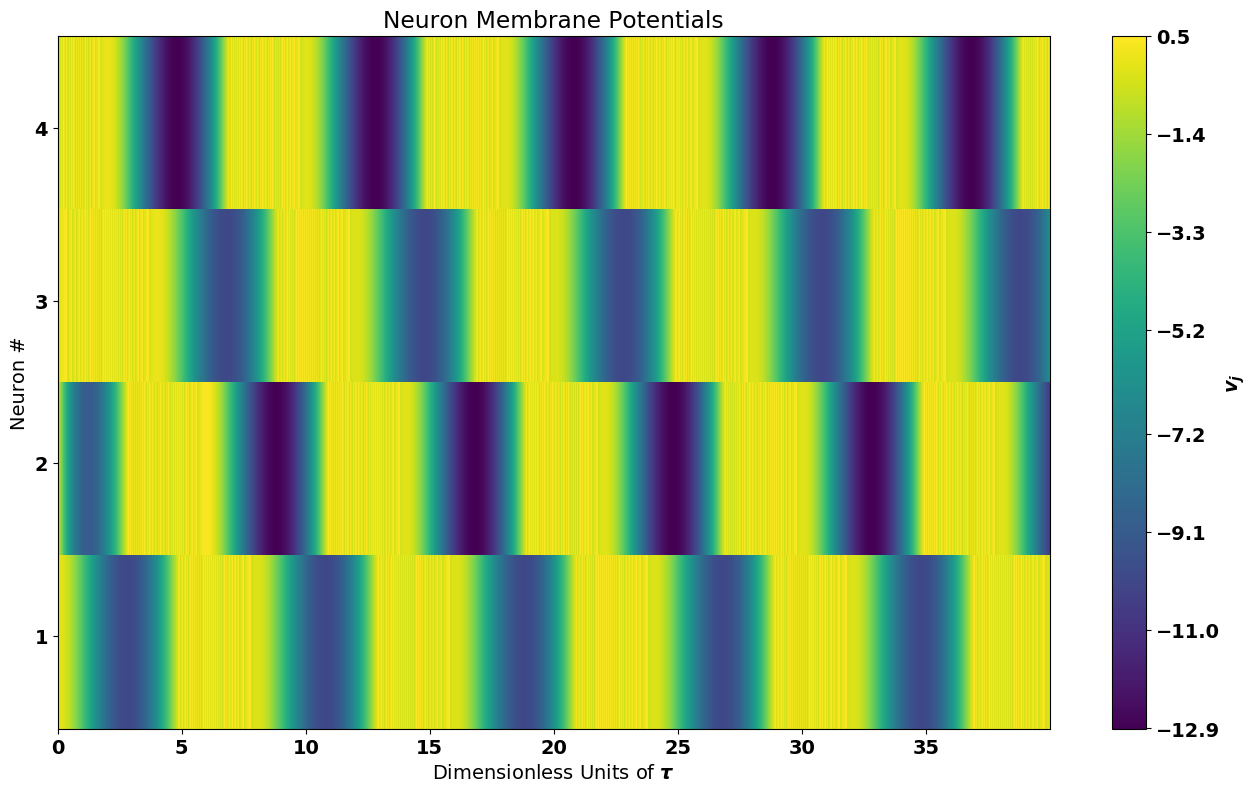
\includegraphics[width=.7\linewidth]{figures/membrane_potential_image.png}
\end{figure}

\newpage

\captionof{figure}{Simulation of equations (\ref{eq:rotated_voltage_dynamics}) and
    (\ref{eq:rho_dot}) with parameters listed in equation (\ref{eq:sim_I_params}). \textbf{\textit{Top:}} The decoded network estimate plotted alongside the target dynamical system. \textbf{\textit{Middle:}} The estimation error along each state-space dimension. \textbf{\textit{Bottom: }}The membrane potentials of the 4 neurons during the same time period.\\
    For the numerical implementation, the matrix exponential was used to integrate the continuous terms over a simulation time step. Continuous terms include all equation terms excepting the delta functions $\Omega$ handled separately. After integrating over a timestep, any neuron above threshold was manually reset (action of fast inhibition). If multiple neurons are above threshold, the system is integrated backwards in time until only one neuron is above threshold before spiking. The matrix exponential was computed using a Pad\'{e} approximation via the Python package Scipy: \textit{scipy.linalg.expm()}. 
    } 
    \label{fig:Simulation_I}